

\chapter{Introduzione}

\section{Presentazione del problema}
Le equazioni differenziali con ritardo sono alla base di molti modelli fisici, ingegneristici e biologici, 
l'interesse per tali problemi è aumentato di recente in seguito allo sviluppo dei computer e all'aumento 
della potenza di calcolo. Un'equazione differeziale con ritardo è della forma
$$
\begin{cases}
 y'(t) = f(t,y(t),y(t- \tau (t,y(t)))	\hspace{1cm}	t_0 \le t \le t_f \\
 y(t)=\phi(t)				\hspace{5cm}	t \le t_0
\end{cases}
$$
Questo è il caso più complesso di equazione differeziale con ritardo, a volte è sufficiente considerare 
il ritardo costante, quindi problemi del tipo
$$
\begin{cases}
 y'(t) = f(t,y(t),y(t- \tau))		\hspace{2cm}	t_0 \le t \le t_f \\
 y(t)=\phi(t)				\hspace{5cm}	t \le t_0
\end{cases}
$$
La funzione $\phi(t)$ è detta storia e nel caso di ritardo constante è sufficiente che il suo 
dominio sia $[t_0-\tau,t_0]$.

\section{Equazione logistica}
Un primo esempio di equazione differeziale con ritardo lo abbiamo nella biologia \cite[pag. 9-13]{1}: nel 
1838 Pierre Francois Verhulst pubblicò un articolo in cui proponeva un modello matematico per 
descrivere la crescita delle popolazioni, tale modello si riassume nella seguente equazione 
differenziale (equazione logistica)
$$
\frac{d N}{d t} = r N(t) \left(1 - \frac{N(t)}{K} \right)
$$
\begin{itemize}
 \item $N$ è il numero di individui della specie
 \item $r$ è il tasso di crescita
 \item $K$ è la capacità di carico della popolazione (numero massimo di individui 
	      che possono trovarsi in un determinato ambiente)
\end{itemize}



La soluzione di tale equazione è
$$
N(t)= \frac{K N_0 e^{rt}}{K+N_0(e^{rt}-1)}
$$

\begin{figure}[ht]
\centering
\caption{Esempio: crescita di Paramecium caudatum $N(4) \simeq K$}
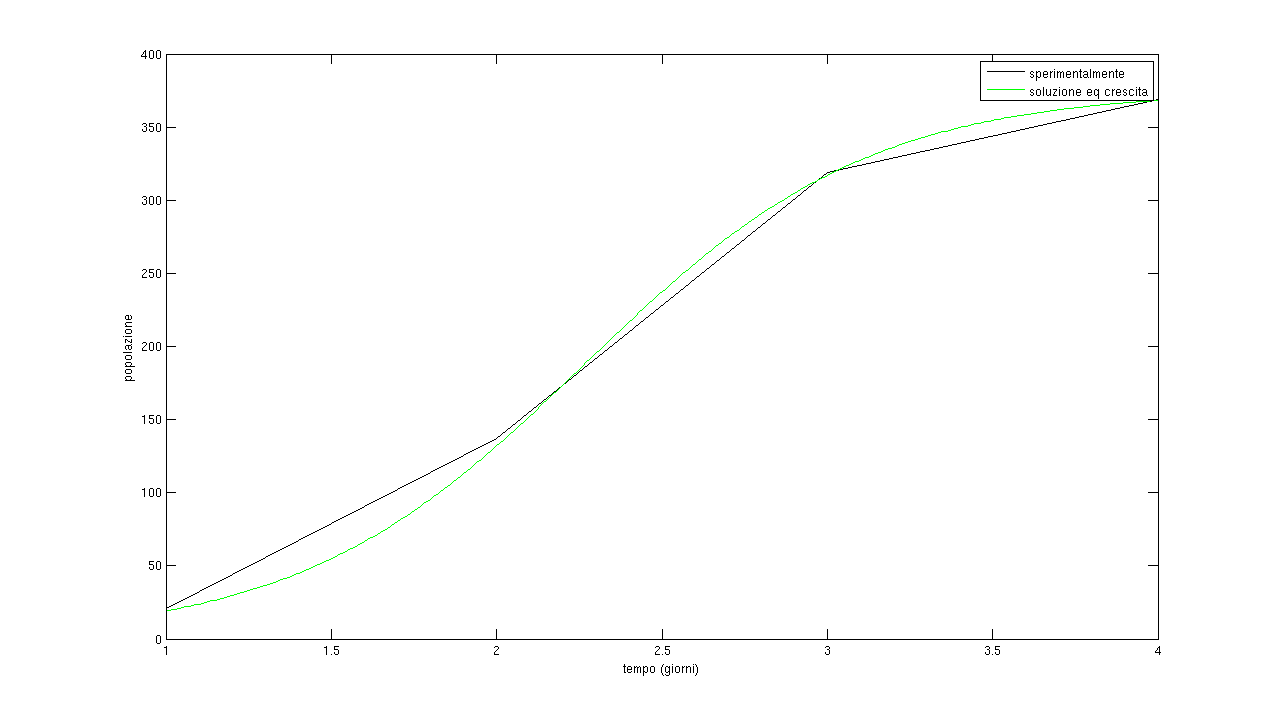
\includegraphics[width=16cm]{immagini/immagine1.png}
\end{figure}

Questa è una funzione crescente e limitata, infatti gli individui tendono a riprodursi 
fino ad arrivare al numero di saturazione $K$, daltronde le misurazioni indicano che il numero di 
individui di alcune specie in alcuni periodi decresce per poi aumentare nuovamente seguendo un adamento 
oscillatorio, quindi nasce l'esigenza di cambiar modello 
oppure di correggere l'attuale. 
L'equazione logistica sottointende che il tasso di nascita/morte degli individi della specie 
risponda istantaneamente ai cambiamenti della dimensione della popolazione daltronde 
ci sono dei casi in cui gli individui di una certa specie sentono l'impulso di 
riprodursi ma non lo fanno subito ma con un certo ritardo, ciò succede se ad esempio 
sono coscienti della disponibilità di cibo oppure possono esser condizionati dall'ambiente. 
Hutchinson fu il primo matematico a introdurre il fattore di ritardo nell'equazione logistica 
per spiegare i fenomeni oscillatori, in tal caso l'equazione diventa
$$
\frac{d N}{d t} = r N(t) \left(1 - \frac{N(t-\tau)}{K} \right)
$$

\begin{exm}
 Supponiamo che il numero massimo di individui di una certa specie che possono esser presenti in un deteminato 
ambiente sia $K=100$, che il tasso di crescita sia del $10 \% $ ovvero $r=0.1$, allora risolvendo l'equazione 
logistica si ottengono risultati diversi in base al ritardo (Figura 1.2). 
\begin{figure}[!ht]
\centering
\caption{Grafici al variare di $\tau$}
\subfigure[$\tau=5$]{
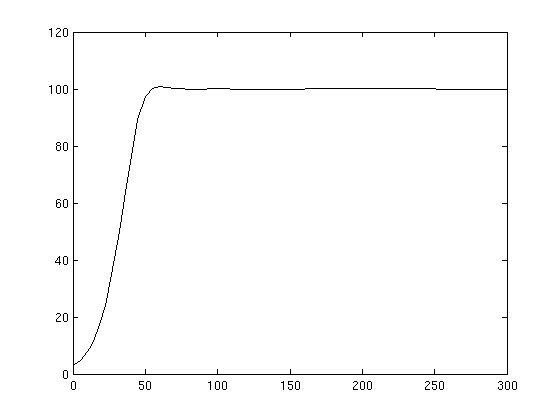
\includegraphics[width=7.2cm]{immagini/immagine2.png}}
\hspace{1mm}
\subfigure[$\tau=10$]{
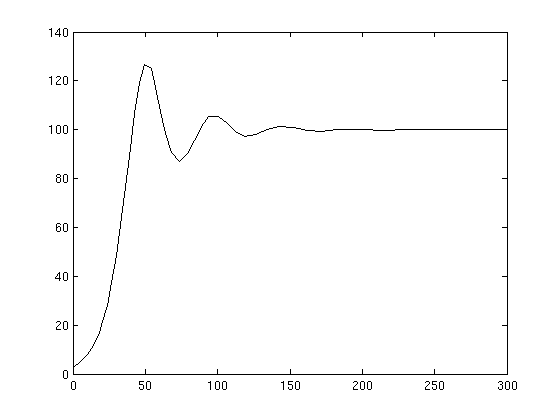
\includegraphics[width=7.2cm]{immagini/immagine3.png}}
\hspace{1mm}
\subfigure[$\tau=20$]{
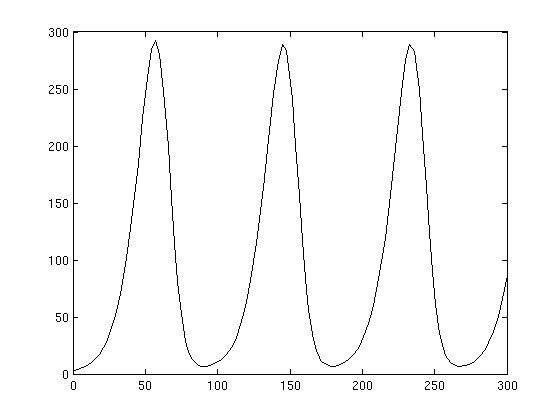
\includegraphics[width=7.2cm]{immagini/immagine4.png}}
\hspace{1mm}
\subfigure[$\tau=27$]{
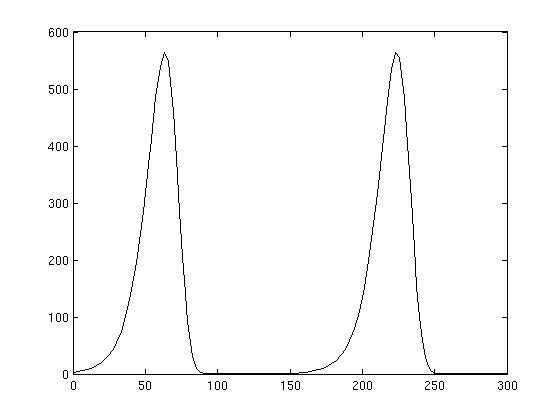
\includegraphics[width=7.2cm]{immagini/immagine5.png}}
\end{figure}
Il ritardo influisce sulla stabilità della soluzione, infatti se $\tau=5$ allora 
il numero di individui cresce fino a stabilizzarsi al numero massimo $K$, quindi il ritardo 
è trascurabile. Se invece $\tau=10$ ci sono delle oscillazioni nei tempi iniziali e dopo la soluzione 
si stabilizza, inoltre il numero di individui supera la capacità massima dell'ambiente.
Se invece $\tau=20$ allora la soluzione non si stabilizza ma oscilla in continuazione, mentre se 
$\tau=27$ allora il ritardo porta all'estinzione delle specie, infatti anche se la soluzione oscilla 
con periodicità dopo il primo picco il numero di abitanti è nullo.
Un esempio pratico del fenomeno appena descritto è dato dalla specie del lemmini (roditori artici) 
che hanno dei cicli, ovvero la popolazione cresce e diminuisce seguendo un andamento oscillatorio 
come nella figura 1.2 (c).
\end{exm}

La tesi tratterà dei metodi numerici che si utilizzano per risolvere le equazioni differenziali 
con ritardo che d'ora in avanti verranno chiamate con l'acronimo DDE (delay differential equation).

